\chapter{Đối xứng trao đổi, spin và hai dấu trừ}

\section{Sự lấp đầy các lớp và câu hỏi về thống kê spin--}

Phần ôn lại mô hình lớp bắt đầu từ hai tính chất gắn với electron. Electron có spin bằng một phần hai, với hai hình chiếu spin không thứ nguyên
\begin{equation}
m_s=+\frac12,
\qquad
m_s=-\frac12,
\end{equation}
và electron tuân theo nguyên lý loại trừ Pauli. Hai sự kiện này có liên quan, nhưng không phải là cùng một mệnh đề.

Cụm từ ``cùng một trạng thái'' cần được hiểu cẩn thận. Không hai electron nào có thể chiếm cùng một trạng thái một hạt đầy đủ. Tuy vậy, hai electron có thể cùng chiếm một orbital không gian nếu trạng thái spin của chúng khác nhau. Trong gần đúng electron độc lập của helium, cả hai electron đều chiếm orbital không gian thấp nhất, một electron spin hướng lên và electron kia spin hướng xuống. Chính xác hơn, hai khả năng ``electron thứ nhất spin hướng lên, electron thứ hai spin hướng xuống'' và ``electron thứ nhất spin hướng xuống, electron thứ hai spin hướng lên'' thuộc về một trạng thái spin vướng víu của hai electron.

Đây chỉ là gần đúng của mô hình lớp cũ. Mô hình bỏ qua tương tác giữa các electron và được dùng để đếm cho đơn giản. Với lithium, hai electron đầu lấp đầy orbital không gian thấp nhất với spin ngược chiều nhau. Electron thứ ba không thể đi vào một trong hai trạng thái đầy đủ ấy, nên phải chiếm một orbital cao hơn.

Bước tiếp theo là sơ đồ quen thuộc của mômen động lượng quỹ đạo. Các phân lớp có
\begin{equation}
\ell=0,\qquad \ell=1,\qquad \ell=2
\end{equation}
được gọi là các trạng thái \(S\), \(P\) và \(D\). Một giá trị cố định của \(\ell\) có
\begin{equation}
2\ell+1
\end{equation}
trạng thái quỹ đạo, nên
\begin{equation}
\ell=0\Rightarrow 1,
\qquad
\ell=1\Rightarrow 3,
\qquad
\ell=2\Rightarrow 5.
\end{equation}
Bài toán Coulomb còn có các suy biến bổ sung: các mức xuyên tâm thuộc những phân lớp \(\ell\) khác nhau có thể có cùng năng lượng. Trong lập luận về sự lấp đầy lớp, lớp kế tiếp chứa một orbital \(S\) và ba orbital \(P\). Vì vậy, lớp này có
\begin{equation}
1+3=4
\end{equation}
trạng thái không gian. Spin làm số trạng thái tăng gấp đôi:
\begin{equation}
2(1+3)=8.
\end{equation}

Tám trạng thái một electron đầy đủ ấy được lấp đầy theo trình tự đơn giản từ lithium đến neon. Sau lớp kín, sodium lại có một electron ở ngoài cùng, đó là lý do bức tranh thô sơ này khiến nó có vẻ giống lithium. Hóa học không phải là đích đến ở đây. Điều cần thấy là spin bán nguyên và nguyên lý loại trừ xuất hiện cùng nhau.

Photon cho thấy sự tương phản. Chúng có spin nguyên và không tuân theo quy tắc loại trừ. Một sóng điện từ cổ điển tương ứng với nhiều photon cùng chiếm một mode. Boson có thể tích tụ trong một trạng thái chung, còn các fermion đồng nhất không thể cùng chiếm một trạng thái đầy đủ quá một lần. Câu hỏi là liệu hai sự ghép cặp ấy có thể ngược lại hay không: spin bán nguyên mà không có nguyên lý loại trừ, hoặc spin nguyên mà vẫn có nguyên lý loại trừ. Trong không gian ba chiều, hệ thức spin--thống kê cho biết là không. Mệnh đề quen thuộc này cần được nêu kèm điều kiện trong một và hai chiều không gian; ở đây không trình bày chứng minh của kết quả trong lý thuyết trường.

\begin{classroomqa}
\lecturetimestamp{00:11:48}
\audiencequestion{Có số lượng tử boson tối đa nào có thể chiếm một trạng thái không?}
\lecturerresponse{Không. Boson không bị giới hạn số hạt chiếm chỗ và có xu hướng tích tụ trong cùng một trạng thái.}
\end{classroomqa}

\section{Hàm sóng nhiều hạt}

Ta sẽ tiếp cận mối liên hệ này qua hai dấu trừ: một dấu do trao đổi, một dấu do phép quay. Hãy bắt đầu với trao đổi và tạm thời bỏ qua spin.

Gọi \(x_i\) là vị trí của hạt \(i\). Chỉ số dưới là nhãn hạt, không phải thành phần Cartesian; ba tọa độ không gian được gói gọn trong ký hiệu \(x_i\) duy nhất. Cơ sở vị trí cho \(n\) hạt là
\begin{equation}
\lvert x_1,x_2,\ldots,x_n\rangle.
\end{equation}
Với một trạng thái trừu tượng \(\lvert\Psi\rangle\), hàm sóng tọa độ là
\begin{equation}
\psi(x_1,x_2,\ldots,x_n)
=
\langle x_1,x_2,\ldots,x_n\mid\Psi\rangle.
\end{equation}
Bình phương độ lớn của nó,
\begin{equation}
\bigl\lvert\psi(x_1,x_2,\ldots,x_n)\bigr\rvert^2,
\end{equation}
là mật độ xác suất đồng thời để tìm hạt \(1\) tại \(x_1\), hạt \(2\) tại \(x_2\), vân vân.

Giờ giả sử các hạt đồng nhất. Trước hết, hãy hình dung một electron được sơn màu xanh lam và một electron khác màu đỏ. Khi đó, ``electron xanh lam ở \(x_1\), electron đỏ ở \(x_2\)'' có thể phân biệt với ``electron xanh lam ở \(x_2\), electron đỏ ở \(x_1\).'' Electron thực không mang những màu sắc hay nhãn riêng như vậy. Đổi chỗ các nhãn dùng để ghi sổ không thể tạo ra một cấu hình vật lý mới.

Một pha tổng thể không làm thay đổi xác suất hay giá trị kỳ vọng. Vì vậy, với một trạng thái thuộc phân lớp trao đổi xác định, hàm sóng tọa độ có thể thỏa mãn
\begin{equation}
\psi(x_2,x_1)=\eta\,\psi(x_1,x_2),
\qquad
\lvert\eta\rvert=1.
\end{equation}
Áp dụng cùng phép trao đổi hai lần sẽ khôi phục các đối số ban đầu và cho
\begin{equation}
\eta^2=1,
\end{equation}
Do đó, hai trị riêng trao đổi có thể có là
\begin{equation}
\eta=+1
\qquad\hbox{or}\qquad
\eta=-1.
\end{equation}

\editorialnote{Đại số của phép trao đổi kép chỉ xác định các trị riêng khả dĩ sau khi đã giả định trạng thái có tính chất trao đổi xác định. Điều kiện bổ sung rằng các trạng thái được phép của một loài nhất định chỉ thuộc về một phân lớp trao đổi là một quy tắc vật lý; nó không suy ra được chỉ từ \(\eta^2=1\). Điều kiện này cũng áp dụng cho lập luận về nguyên lý loại trừ bên dưới: tính phản đối xứng kéo theo nguyên lý loại trừ sau khi đã chọn phân lớp fermion, nhưng riêng đại số của phép trao đổi không chọn ra phân lớp ấy.}

Với boson, các hàm sóng được phép là đối xứng,
\begin{equation}
\psi_B(x_1,x_2)=\psi_B(x_2,x_1),
\end{equation}
còn với fermion, chúng phản đối xứng,
\begin{equation}
\psi_F(x_1,x_2)=-\psi_F(x_2,x_1).
\end{equation}
Dấu trừ không thể nhận thấy khi nó nhân với toàn bộ trạng thái, nhưng lại quan trọng khi cộng các biên độ. Đó là cách đối xứng trao đổi tạo ra những hệ quả quan sát được.

\section{Tích, tổng và nguyên lý loại trừ}

Trước hết, xét hai hạt được gán vào cùng một orbital một hạt \(\psi_0\). Tích của chúng là
\begin{equation}
\psi_0(x_1)\psi_0(x_2).
\end{equation}
Đổi chỗ tọa độ hạt cho kết quả
\begin{equation}
\psi_0(x_2)\psi_0(x_1)
=
\psi_0(x_1)\psi_0(x_2).
\end{equation}
Giá trị của hàm sóng là các số, không phải toán tử, nên các thừa số giao hoán. Tích ứng với cùng trạng thái là đối xứng. Đây là dạng được phép đối với boson, nhưng không thể mô tả hai fermion đồng nhất.

Tiếp theo, gán các hạt vào những orbital một hạt khác nhau:
\begin{equation}
\psi_0(x_1)\psi_1(x_2).
\end{equation}
Phép trao đổi cho
\begin{equation}
\psi_0(x_2)\psi_1(x_1).
\end{equation}
Với hai hàm khác nhau, tích sau khi đổi chỗ nói chung không bằng biểu thức ban đầu cũng không bằng số đối của nó. Vì vậy, tích đơn thuần không có tính đối xứng trao đổi cần thiết nào. Điều này không cấm một hạt chiếm \(\psi_0\) trong khi hạt kia chiếm \(\psi_1\). Có nghĩa là trạng thái hai hạt phải kết hợp hai cách gán ấy.

Tổ hợp đối xứng là
\begin{equation}
\psi_B^{(01)}(x_1,x_2)
\propto
\psi_0(x_1)\psi_1(x_2)
+
\psi_0(x_2)\psi_1(x_1),
\end{equation}
còn tổ hợp phản đối xứng là
\begin{equation}
\psi_F^{(01)}(x_1,x_2)
\propto
\psi_0(x_1)\psi_1(x_2)
-
\psi_0(x_2)\psi_1(x_1).
\end{equation}
Các dấu tỉ lệ là đủ dùng vì lập luận về trao đổi không cần chuẩn hóa. Cả hai trạng thái đều có một hạt trong mỗi orbital; chúng chỉ khác nhau ở cách kết hợp hai cách gán không thể phân biệt.

Giờ cho hai orbital trùng nhau. Tổ hợp boson trở thành
\begin{align}
\psi_B^{(00)}(x_1,x_2)
&\propto
\psi_0(x_1)\psi_0(x_2)
+
\psi_0(x_2)\psi_0(x_1)\\
&=
2\psi_0(x_1)\psi_0(x_2),
\end{align}
và khác không. Tổ hợp fermion cho
\begin{align}
\psi_F^{(00)}(x_1,x_2)
&\propto
\psi_0(x_1)\psi_0(x_2)
-
\psi_0(x_2)\psi_0(x_1)\\
&=0.
\end{align}
Với quy tắc trao đổi phản đối xứng, nguyên lý loại trừ được suy ra: không tồn tại trạng thái phản đối xứng khác không mà trong đó cả hai fermion cùng ở một trạng thái một hạt.

Đối với trạng thái nhiều hạt, quy tắc này áp dụng cho mọi phép chuyển vị của hai đối số. Phép chuyển vị giữ nguyên hàm sóng boson và đảo dấu hàm sóng fermion. Lặp lại cùng phép chuyển vị thì trong cả hai trường hợp đều trở về như cũ. Điều gây ngạc nhiên là một phép trao đổi đơn lẻ, dù không làm thay đổi nhãn hạt có thể quan sát, lại đổi dấu trạng thái fermion.

\section{Spin trong nhãn đầy đủ của hạt}

Giờ có thể đưa spin trở lại với một thay đổi nhỏ. Biên độ một hạt phụ thuộc vào cả vị trí lẫn nhãn spin rời rạc,
\begin{equation}
\psi(x,\sigma),
\end{equation}
trong đó \(\sigma=+1\) hoặc \(-1\) là nhãn cho kết quả \(\sigma_z\) đã chọn. Bình phương độ lớn là mật độ xác suất đồng thời ứng với vị trí và nhãn spin đã nêu.

Với nhiều hạt, hàm sóng là
\begin{equation}
\psi(x_1,\sigma_1;\,x_2,\sigma_2;\,\ldots).
\end{equation}
Phép trao đổi hoán đổi mọi thứ thuộc về hai hạt, chứ không chỉ vị trí của chúng:
\begin{align}
\psi_B(x_1,\sigma_1;\,x_2,\sigma_2)
&=
+\psi_B(x_2,\sigma_2;\,x_1,\sigma_1),\\
\psi_F(x_1,\sigma_1;\,x_2,\sigma_2)
&=
-\psi_F(x_2,\sigma_2;\,x_1,\sigma_1).
\end{align}
Đây là dạng chính xác của phát biểu mở đầu về mô hình lớp. Hai electron chỉ có thể cùng chiếm một orbital không gian khi các trạng thái đầy đủ của chúng, bao gồm cả spin, khác nhau.

\begin{classroomqa}
\lecturetimestamp{00:34:33}
\audiencequestion{Đối xứng trao đổi có phải là một trường hợp của nhóm hoán vị không?}
\lecturerresponse{Đúng. Trao đổi các hạt là một phép hoán vị, và quy luật biến đổi với dấu cộng hoặc dấu trừ tạo thành một biểu diễn của nhóm hoán vị.}
\end{classroomqa}

\begin{classroomqa}
\lecturetimestamp{00:35:12}
\audiencequestion{Tại sao trong phép dựng trạng thái hai hạt lại dùng tích thay vì tổng các hàm sóng một hạt?}
\lecturerresponse{Tổng mô tả một hạt ở trạng thái chồng chập. Tích thuộc không gian tích tensor hai hạt và mô tả mỗi hạt được gán vào một trạng thái một hạt.}
\end{classroomqa}

Phép trao đổi nhãn đầy đủ được minh họa trên bảng bên dưới.\footnote{Thứ tự của các nhãn vị trí--spin được khôi phục từ khung hình bảng đen còn đọc được và phần giải thích xung quanh, từ 00:33:43 đến 00:34:25.}
\begin{figure}[htbp]
\centering
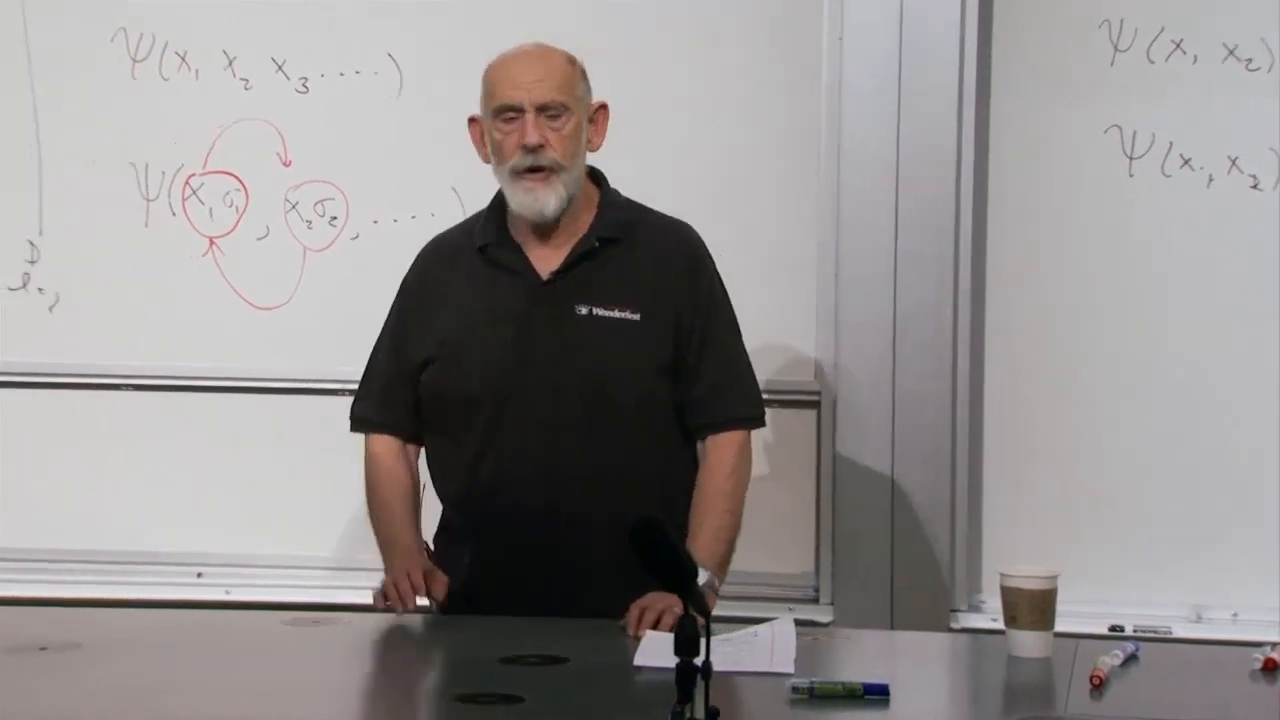
\includegraphics[width=0.9\linewidth]{lecture_05_frame_03.png}
\caption{Trao đổi hai hạt đồng nhất làm hoán đổi các nhãn vị trí--spin đầy đủ của chúng. Trạng thái boson không đổi, còn trạng thái fermion đổi dấu.}
\lectureframe{00:35:25}
\end{figure}

Đây là hai cách dùng tính tuyến tính khác nhau. Với một hạt,
\begin{equation}
\alpha\psi_0(x)+\beta\psi_1(x)
\end{equation}
là trạng thái chồng chập của hai khả năng. Với hai hạt,
\begin{equation}
\psi_0(x_1)\psi_1(x_2)
\end{equation}
là một biên độ tích trong không gian có hai tọa độ hạt. Phép đối xứng hóa hoặc phản đối xứng hóa kết hợp tích ấy với tích tương ứng sau khi trao đổi.

\begin{classroomqa}
\lecturetimestamp{00:36:13}
\audiencequestion{Trao đổi các hạt có tạo ra hiệu ứng giao thoa không?}
\lecturerresponse{Có. Biên độ fermion cùng trạng thái bằng không có thể được hiểu là giao thoa triệt tiêu giữa hai đóng góp sau khi trao đổi.}
\end{classroomqa}

\begin{classroomqa}
\lecturetimestamp{00:37:13}
\audiencequestion{Pauli có suy ra nguyên lý loại trừ bằng chính lập luận đối xứng này không?}
\lecturerresponse{Pauli bắt đầu từ một sự kiện thực nghiệm và tìm ra khuôn khổ toán học để diễn đạt nó. Ban đầu, ông không suy ra nguyên lý loại trừ từ một lý thuyết nền tảng hơn.}
\end{classroomqa}

Tính phản đối xứng cung cấp khuôn khổ toán học để diễn đạt quy tắc loại trừ thực nghiệm.

\begin{classroomqa}
\lecturetimestamp{00:39:01}
\audiencequestion{Giao thoa do trao đổi hạt có liên hệ với giao thoa giữa các đường đi khả dĩ không?}
\lecturerresponse{Có. Trong một lịch sử, hai hạt đi qua mà không cắt nhau; trong lịch sử kia, chúng cắt nhau để đến các đích đã hoán đổi. Các biên độ cộng lại với boson và có thể triệt tiêu với fermion.}
\end{classroomqa}

Phép trao đổi tạo ra dấu trừ thứ nhất. Phép quay tạo ra dấu trừ thứ hai.

\section{Dấu trừ thứ hai: phép quay một góc \texorpdfstring{\(2\pi\)}{2 pi}}

Một vòng quay trọn vẹn có vẻ như chẳng làm gì. Mọi hướng hình học thông thường đều trở về vị trí ban đầu sau một góc \(2\pi\). Tuy nhiên, điều cần trở về như cũ là xác suất và giá trị kỳ vọng. Bản thân vectơ trạng thái có thể trở về cùng với một pha tổng thể, giống như trong phép trao đổi.

\begin{classroomqa}
\lecturetimestamp{00:42:12}
\audiencequestion{Phép quay được thực hiện quanh trục nào, và toán tử sinh là mômen động lượng quỹ đạo, spin hay cả hai?}
\lecturerresponse{Có thể chọn một trục bên ngoài; dưới đây ta chọn trục \(z\). Toán tử sinh là mômen động lượng toàn phần, bao gồm cả phần quỹ đạo lẫn phần spin. Bản thân spin không nhất thiết phải hướng dọc theo trục đã chọn.}
\end{classroomqa}

\editorialnote{Các công thức mômen động lượng trong phần thảo luận này dùng đơn vị \(\hbar=1\), vì thế \(m\) là trị riêng không thứ nguyên của \(J_z\).}

Gọi \(\psi(\theta)\) là trạng thái thu được khi tham số quay tăng dần qua một góc \(\theta\). Theo quy ước dùng ở đây,
\begin{equation}
J_z\psi(\theta)
=
-i\frac{\partial}{\partial\theta}\psi(\theta).
\end{equation}
Với trạng thái có \(J_z\) xác định,
\begin{equation}
J_z\psi(\theta)=m\psi(\theta).
\end{equation}
Kết hợp các phương trình ta được
\begin{equation}
-i\frac{\partial}{\partial\theta}\psi(\theta)
=
m\psi(\theta),
\end{equation}
nghiệm là
\begin{equation}
\psi(\theta)=e^{im\theta}\psi(0).
\end{equation}

Các giá trị được phép của \(m\) là số nguyên hoặc bán nguyên. Do đó,
\begin{equation}
\psi(2\pi)
=
\begin{cases}
+\psi(0), & m\in\mathbb Z,\\[4pt]
-\psi(0), & m\in\mathbb Z+\tfrac12.
\end{cases}
\end{equation}
Sau thêm một vòng quay trọn vẹn,
\begin{equation}
\psi(4\pi)=\psi(0)
\end{equation}
trong cả hai trường hợp. Đây là dấu trừ thứ hai: trạng thái thuộc một đa tuyến mômen động lượng bán nguyên đổi dấu dưới phép quay góc \(2\pi\).

Dấu này không làm thay đổi \(\lvert\psi\rvert^2\), nên không thể quan sát được khi nó nhân với toàn bộ trạng thái. Dù vậy, phép quay góc \(2\pi\) không được biểu diễn bằng toán tử đơn vị trên trạng thái spin bán nguyên. Khác biệt này trở nên quan sát được khi dấu ấy tương đối với một biên độ kết hợp khác.

\section{Các đường đi quay góc \texorpdfstring{\(2\pi\) và \(4\pi\)}{2 pi và 4 pi}}

Có thể làm lộ rõ khác biệt giữa \(2\pi\) và \(4\pi\) mà không cần thêm đại số. Cầm một chiếc cốc bằng một tay rồi xoay trọn một vòng mà không buông tay. Cốc trở lại hướng ban đầu, nhưng cánh tay bị xoắn. Xoay tiếp thêm một vòng nữa thì có thể đưa cánh tay về vị trí ban đầu mà không phải đảo ngược chuyển động của cốc.

Một cách dựng liên quan là đặt một quả cầu trong hộp rồi nối nó với hộp bằng các sợi dây. Xoay quả cầu một góc \(2\pi\) sẽ làm dây rối. Trong không gian ba chiều thông thường, có thể gỡ rối dây ứng với một vòng quay \(4\pi\). Đối tượng cần xét không chỉ là hướng cuối cùng của quả cầu mà còn là đường đi qua không gian các phép quay.

\begin{classroomqa}
\lecturetimestamp{00:54:22}
\audiencequestion{Nếu xoay quả cầu hai vòng quanh cùng một trục thì có thể gỡ rối dây thật không? Việc đó có cần thêm một chiều không gian không?}
\lecturerresponse{Có thể gỡ rối đường đi \(4\pi\) trong không gian ba chiều thông thường. Thời gian tham số hóa chuyển động; nó không phải là một hướng không gian khác. Không thể gỡ rối đường đi \(2\pi\) theo cách này, trong khi có thể gỡ rối đường đi \(4\pi\).}
\end{classroomqa}

Các minh họa phân biệt đường đi \(2\pi\) không tầm thường với đường đi \(4\pi\) có thể gỡ rối, mà không triển khai lý thuyết hình thức về nhóm quay.

\section{Trao đổi và phép quay trong hình ảnh dây đai}

Giờ hai dấu trừ được đặt cạnh nhau. Trao đổi hai fermion đồng nhất làm đổi dấu hàm sóng chung của chúng. Quay một trạng thái spin bán nguyên một góc \(2\pi\) cũng làm đổi dấu trạng thái. Dây đai cho thấy mối liên hệ hình học giữa hai phép biến đổi.

Sắp xếp dây đai sao cho hai đầu dưới của nó đã bị hoán đổi. Nhìn theo cách khác, chính dây đai ấy có một vòng xoắn \(2\pi\). Thực hiện phép trao đổi cùng với phép quay \(2\pi\) sẽ xóa vòng xoắn và để lại dây đai không xoắn. Có thể liên tục biến quá trình kết hợp này về trạng thái không làm gì.\footnote{Trong bài giảng, nhận xét về phép trao đổi--quay được quy cho David Finkelstein. Tư liệu nguồn không nêu ấn phẩm cụ thể nào, nên ở đây tên ông chỉ được giữ lại như một sự quy thuộc.}

\begin{classroomqa}
\lecturetimestamp{01:01:12}
\audiencequestion{Đây chỉ là mệnh đề về cách dây đai nằm trong không gian, chứ không phải mệnh đề về tô pô của hạt, phải không?}
\lecturerresponse{Có thể xem dây đai như lịch sử của hạt trong không thời gian. Khi thời gian tăng theo chiều hướng lên, mặt cắt ngang của nó cho ta các vật thể kiểu hạt. Một cặp được tạo ra, một vật thể quay góc \(2\pi\), rồi hai vật thể đồng nhất được trao đổi. Trong lịch sử đó, các pha do phép quay và phép trao đổi triệt tiêu nhau.}
\end{classroomqa}

Lịch sử này làm rõ việc theo dõi pha. Bắt đầu khi chưa có hạt nào. Tại hai vị trí cách xa nhau, tạo ra một cặp hạt--phản hạt, để lại bốn hạt ở một thời điểm trung gian. Quay một hạt góc \(2\pi\) đồng thời trao đổi hai hạt đồng nhất khác trong cấu hình. Có thể biến dạng toàn bộ lịch sử này thành lịch sử sơ cấp, trong đó một cặp được tạo ra rồi sau đó hủy. Theo cách theo dõi dấu đang bàn đến, lịch sử tầm thường ấy không có pha bổ sung. Nếu \(\eta_{\mathrm{rot}}\) và \(\eta_{\mathrm{ex}}\) lần lượt là hai dấu, sự triệt tiêu được nêu bằng lời có thể viết gọn thành\footnote{Phương trình pha này ghi lại sự triệt tiêu được mô tả từ 01:06:50 đến 01:07:18; bài giảng trình bày phép dựng này như một gợi ý, chứ không phải một chứng minh nghiêm ngặt.}
\begin{equation}
\eta_{\mathrm{rot}}\eta_{\mathrm{ex}}=1.
\end{equation}

\begin{classroomqa}
\lecturetimestamp{01:03:34}
\audiencequestion{Có thể liên hệ phép trao đổi với phép quay bằng cách cho mỗi hạt trong hai hạt chuyển động một góc \(\pi\) rồi định hướng lại chúng không?}
\lecturerresponse{Cách dựng đó có thể phản ánh toán học liên quan, nhưng nó dùng hai phép quay riêng biệt, mỗi phép một góc \(\pi\). Quá trình đang phân tích ở đây chỉ có một phép quay góc \(2\pi\), nên hai lập luận không đồng nhất.}
\end{classroomqa}

Lập luận này dựa vào khả năng tạo ra và hủy các vật thể kiểu hạt. Nó sẽ không có dạng này trong một lý thuyết mà các hạt tồn tại vĩnh viễn. Lập luận cũng không được đưa ra như chứng minh chuẩn của định lý spin--thống kê. Mục đích của nó là chỉ ra một lý do tô pô khiến các dấu do trao đổi và phép quay tương thích với nhau.

\section{Các cấu hình cục bộ, ảnh gương và sự hủy}

Có thể lặp lại phép dựng này với các cấu hình trường định xứ. Giả sử một hay nhiều trường nhận giá trị chân không ở hầu hết mọi nơi, nhưng có hình dạng và cấu trúc khác không trong một vùng nhỏ. Cấu hình định xứ ấy là một cấu hình dạng cục.

Giờ tạo cấu hình thứ hai là ảnh gương thích hợp của cấu hình thứ nhất. Gọi một cấu hình là hạt và cấu hình kia là phản hạt. Đưa chúng lại gần nhau. Các phần tương ứng của hai cấu hình trường gặp nhau và triệt tiêu lẫn nhau. Ở một giai đoạn trung gian, một số phần của các cấu hình dạng cục có thể đã biến mất trong khi những phần khác vẫn còn. Tiếp tục biến dạng sẽ xóa cấu trúc còn lại và đưa các trường trở về cấu hình chân không. Hai vòng xoắn ngược chiều trong dây đai cho ta cùng hình ảnh: đẩy chúng lại gần nhau, chúng sẽ tháo xoắn.

Có thể chạy quá trình này theo chiều ngược lại. Không gian trống có thể sinh ra một cấu hình dạng cục cùng ảnh gương của nó. Ta có thể tạo hai cặp như vậy, quay một cấu hình dạng cục một góc \(2\pi\), trao đổi hai cấu hình dạng cục đồng nhất rồi lại hủy các cặp. Khi đó, sự triệt tiêu giữa phép trao đổi--quay vẫn áp dụng. Đây vẫn là phần mở rộng mang tính trực giác của phép dựng, chứ không phải định lý về mọi kích thích định xứ.

\begin{classroomqa}
\lecturetimestamp{01:11:30}
\audiencequestion{Có hiện thực vật lý nào của những cấu hình trường dạng cục này không?}
\lecturerresponse{Có. Ví dụ gồm hạt nhân trong mô tả kiểu Skyrmion, đơn cực từ và các kích thích trường khác có tính chất như hạt.}
\end{classroomqa}

Hình ảnh các cấu hình dạng cục cùng ảnh gương giúp ta hiểu được phép khái quát hóa. Điều quan trọng không phải là vật thể ban đầu có phải hạt điểm sơ cấp hay không, mà là một kích thích kiểu hạt và đối tác của nó có thể được tạo ra, đưa lại gần nhau rồi hủy một cách liên tục. Đặc điểm đó gợi mở một mối liên hệ rộng hơn giữa phép quay và hành vi trao đổi.

\begin{classroomqa}
\lecturetimestamp{01:16:12}
\audiencequestion{Spin bằng một phần hai có nghĩa là trạng thái chỉ tích lũy một nửa pha quay thông thường phải không?}
\lecturerresponse{Pha theo quy ước này là \(e^{im\theta}\). Với \(m\) bán nguyên, phép quay góc \(2\pi\) cho \(-1\), còn phép quay góc \(4\pi\) cho \(+1\).}
\end{classroomqa}

\section{Dấu tổng thể và thí nghiệm cho kết quả không}

Có thể quan sát dấu trừ do phép quay góc \(2\pi\) không? Trước hết, hãy xét một thí nghiệm mà trong đó không thể quan sát dấu ấy. Giam một electron trong từ trường, để spin của nó đi theo từ trường khi thiết bị được quay chậm một góc \(2\pi\), rồi thả electron vào một thiết bị giao thoa. So sánh với quy trình tương tự nhưng không có phép quay.

Phép quay làm trạng thái biến đổi theo
\begin{equation}
\psi\longmapsto-\psi,
\end{equation}
nhưng dấu trừ nhân với toàn bộ trạng thái. Mọi xác suất đều không đổi, nên mẫu giao thoa cuối cùng không lưu lại dấu vết nào cho biết phép quay sơ bộ có diễn ra hay không. Đây là một thí nghiệm cho kết quả không: pha chung không có gì để giao thoa với nó.

\begin{classroomqa}
\lecturetimestamp{01:20:01}
\audiencequestion{Tại sao phải quay từ trường thật chậm?}
\lecturerresponse{Spin phải tiếp tục đi theo từ trường đang quay. Nếu kéo từ trường quay quá nhanh, spin sẽ không còn duy trì được sự khóa hướng theo nó.}
\end{classroomqa}

\section{Một electron trong hai nhánh kết hợp}

Dấu này trở nên quan sát được khi xét tương đối. Cho một electron đi qua bộ tách chùm. Một phần hàm sóng đi theo đường này, phần còn lại đi theo đường kia:
\begin{equation}
\psi(x)=\psi_1(x)+\psi_2(x).
\end{equation}
Đây là một electron, không phải hai electron. Nó ở trạng thái chồng chập kết hợp của hai khả năng. Cần phân biệt rõ: hai bó sóng không phải là hai hạt độc lập.

Dẫn hai bó sóng vào những vùng riêng biệt có chứa từ trường. Quay từ trường ở một vùng góc \(2\pi\), còn vùng kia giữ nguyên. Với trạng thái spin bán nguyên,
\begin{equation}
\psi_1(x)+\psi_2(x)
\longmapsto
\psi_1(x)-\psi_2(x),
\end{equation}
trong đó nhánh bị quay được gán nhãn \(2\). Giờ dấu này là tương đối. Khi hai bó sóng chồng lấp trở lại, phép cộng trở thành phép trừ. Một điểm giao thoa tăng cường có thể trở thành điểm giao thoa triệt tiêu, thậm chí là một nút.

\begin{classroomqa}
\lecturetimestamp{01:23:46}
\audiencequestion{Nếu chỉ có một electron nhưng hai nhánh hàm sóng, thì cái gì đang được quay?}
\lecturerresponse{Electron ở trạng thái chồng chập kết hợp của hai khả năng định xứ. Một nhánh được quay, nhánh kia thì không. Nếu mở các hộp để biết khả năng nào đã xảy ra, phép đo ấy sẽ phá hủy giao thoa.}
\end{classroomqa}

Mở các hộp ra chỉ cho biết electron duy nhất nằm trong hộp này hay hộp kia. Nếu không thực hiện phép đo đó, cả hai biên độ vẫn còn trong trạng thái. Lặp lại thí nghiệm sẽ tích lũy mẫu giao thoa, mỗi lần phát hiện một electron. Tại nút do dấu trừ tương đối tạo ra, không phát hiện được electron nào.

\section{Tiền động từ và giao thoa hai khe}

Một bố trí sơ đồ thực tế hơn thay cho thí nghiệm với chiếc hộp cần thời gian rất lâu. Tách một sóng electron kết hợp thành hai đường đi. Trên một đường, cho electron đi qua vùng từ trường khi spin ban đầu vuông góc với từ trường. Khi đó spin tiến động. Bằng cách chọn cường độ từ trường và thời gian bay, có thể làm spin ở nhánh đó quay trọn một vòng \(2\pi\), trong khi nhánh kia không trải qua phép quay như vậy.\footnote{Bài giảng nói rằng một thí nghiệm liên quan đến pha spinor đã được thực hiện và mô tả nguyên lý của thí nghiệm, nhưng tư liệu nguồn không xác định bài báo hay thiết bị cụ thể. Vì vậy, phần trình bày ở đây chỉ giới hạn ở phép dựng được nêu trong bài giảng.}

\begin{classroomqa}
\lecturetimestamp{01:27:05}
\audiencequestion{Làm sao xác định được đường đi của electron đơn lẻ?}
\lecturerresponse{Không thể xác định mà không làm hỏng thí nghiệm. Bất kỳ phép đo nào ghi lại đường đi của electron đều phá hủy giao thoa.}
\end{classroomqa}

\begin{classroomqa}
\lecturetimestamp{01:27:50}
\audiencequestion{Chính xác thì một nhánh của hàm sóng là gì, và bộ tách chùm tạo ra hai nhánh bằng cách nào?}
\lecturerresponse{Nhánh là một bó sóng định xứ dọc theo một đường đi. Bộ tách biến sóng tới thành hai bó sóng tách biệt trong không gian; các trường điện hoặc từ có thể dẫn chúng theo những đường khác nhau.}
\end{classroomqa}

Ngoài vùng từ trường, đây là thí nghiệm hai khe. Sóng electron tới tách thành hai bó sóng. Các sóng đi ra lan rộng vào một vùng phát hiện chung, nơi các biên độ chồng lấp. Nếu không có phép quay tương đối, các biên độ ở tâm có thể cộng lại. Phép quay spin góc \(2\pi\) trên một đường đi đảo dấu một biên độ và có thể làm các đóng góp tương ứng triệt tiêu nhau.

\begin{classroomqa}
\lecturetimestamp{01:30:46}
\audiencequestion{Nếu electron đi qua các ống hay khe riêng biệt, làm sao có thể xảy ra giao thoa?}
\lecturerresponse{Phép phát hiện cuối cùng không cho biết đường đi. Hai biên độ sóng đi ra lan rộng và chồng lấp tại đầu dò. Quan sát để biết hạt đã đi theo đường nào sẽ phá hủy giao thoa.}
\end{classroomqa}

\begin{classroomqa}
\lecturetimestamp{01:33:22}
\audiencequestion{Đường kính ống hay khe có phải xấp xỉ bước sóng electron không?}
\lecturerresponse{Với một cách hiện thực hóa thí nghiệm hai khe dựa đúng nghĩa vào nhiễu xạ, khe mở phải đủ nhỏ để tạo ra độ lan rộng cần thiết. Thiết bị đang mô tả chỉ mang tính sơ đồ, không phải một thiết kế thực dụng.}
\end{classroomqa}

\begin{classroomqa}
\lecturetimestamp{01:33:44}
\audiencequestion{Liệu phép quay phân cực của photon một góc tương ứng với \(2\pi\) có khiến hình giao thoa không thay đổi?}
\lecturerresponse{Có. Photon có spin nguyên, nên một phép quay trọn vẹn \(2\pi\) không tạo ra dấu trừ fermion.}
\end{classroomqa}

\begin{classroomqa}
\lecturetimestamp{01:34:12}
\audiencequestion{Thí nghiệm thực tế khác phiên bản lý tưởng hóa ở điểm nào?}
\lecturerresponse{Trong cách dựng lý tưởng, spin được quay đoạn nhiệt. Theo mô tả thực tế, electron chuyển động qua một vùng từ trường và spin của nó tiến động nhanh hơn, nhưng pha đo được vẫn là pha ứng với một vòng quay \(2\pi\).}
\end{classroomqa}

Cách dựng chậm làm nổi bật ý tưởng bằng cách bảo đảm spin đi theo từ trường mà không có chuyển động bổ sung. Cách dựa trên sự tiến động tạo ra cùng dấu tương đối nhờ động lực học. Dù dùng cách nào, hai đường đi phải không còn phân biệt được thì mới có thể xuất hiện hình giao thoa.

\begin{classroomqa}
\lecturetimestamp{01:36:15}
\audiencequestion{Sau bộ tách, có cần cho hai nhánh kết hợp lại không?}
\lecturerresponse{Có. Các gói sóng đi ra phải chồng lấp lên nhau hoặc trải rộng trên cùng một vùng ghi nhận, để biên độ của chúng có thể tạo thành hình giao thoa.}
\end{classroomqa}

\begin{classroomqa}
\lecturetimestamp{01:38:12}
\audiencequestion{Thí nghiệm quay một electron này có phải là hệ quả của nguyên lý loại trừ Pauli không?}
\lecturerresponse{Không. Ở đây chỉ có một electron. Thí nghiệm đo pha spinor khi quay, chứ không đo sự loại trừ hai fermion khỏi cùng một trạng thái.}
\end{classroomqa}

\section{Giao thoa do trao đổi và phép quay tương đối}

Có thể làm lộ dấu trao đổi bằng cùng một phương pháp tổng quát, dù thiết bị được đề xuất phức tạp hơn. Bắt đầu với hai electron và tách hàm sóng chung của chúng thành hai nhánh kết hợp. Vẫn chỉ có hai electron, chứ không phải bốn: cặp electron đi theo một phương án hoặc phương án kia. Ở một nhánh, hoán đổi hai electron; ở nhánh còn lại, giữ nguyên thứ tự của chúng. Sau khi hai nhánh được đưa lại với nhau, dấu trao đổi fermion xuất hiện dưới dạng pha tương đối và có thể làm thay đổi giao thoa.

Đề xuất cuối cùng so sánh trực tiếp hai dấu trừ. Một nhánh nhận pha trao đổi fermion, còn nhánh kia nhận pha tương ứng với phép quay \(2\pi\). Cả hai pha đều bằng \(-1\), nên hiệu ứng tương đối triệt tiêu.\footnote{Bản ghi trong khoảng từ 01:40:26 đến 01:41:15 cho thấy rõ pha trao đổi, pha của phép quay \(2\pi\) và sự triệt tiêu của chúng, nhưng không thể xác định từ phần lời nói hiện có phép quay được gán cụ thể như thế nào.} Bài giảng trình bày đây là một thí nghiệm tư tưởng được đề xuất và cho biết, theo hiểu biết của người nói, thí nghiệm này chưa từng được thực hiện.

\begin{classroomqa}
\lecturetimestamp{01:41:34}
\audiencequestion{Việc quan sát thấy pha trao đổi có thách thức tính không thể phân biệt của hai electron không?}
\lecturerresponse{Không. Tính không thể phân biệt trong cơ học lượng tử tinh tế hơn sự đồng nhất theo nghĩa cổ điển. Nó cho phép vectơ trạng thái đổi dấu khi trao đổi, dù không có nhãn quan sát được nào phân biệt các hạt.}
\end{classroomqa}

Còn một điểm cần lưu ý cuối cùng. Quay toàn bộ một thế giới cô lập qua \(2\pi\) chỉ tạo ra một pha chung, và không thí nghiệm nội tại nào có thể phát hiện được pha đó. Thí nghiệm có thể phát hiện được là phép quay một nhánh kết hợp tương đối với nhánh kia. Vì vậy, điều được quan sát không phải là một dấu tuyệt đối, mà là giao thoa do một dấu tương đối tạo ra.
